\documentclass[14pt, a4paper]{article}
\usepackage[russian]{babel}
\usepackage{graphicx}
\usepackage{layout}
\usepackage[14pt]{extsizes}

\usepackage{xcolor}
\usepackage{hyperref}

 % Цвета для гиперссылок
\definecolor{linkcolor}{HTML}{000000} % цвет ссылок
\definecolor{urlcolor}{HTML}{000000} %цвет гиперссылок

\hypersetup{pdfstartview=FitH,  linkcolor=linkcolor,urlcolor=urlcolor, colorlinks=true}

\oddsidemargin = 0pt
\marginparwidth = 45pt %57
\textwidth = 467pt
\textheight = 716pt
\topmargin = 0pt %17
\footskip = 30pt %30
\headheight = 0pt %12
\headsep = 0pt %25

\begin{document}

\begin{titlepage}
    \topmargin=216pt
    \newpage
    \hangindent=0.7cm
    \huge ИУ-10\\
    Системное\\
    Программное\\
    Обеспечение\\
    \textbf{Введение в виртуализацию}

    \vspace{10cm}

    \begin{center}
        \small\textit{Москва, 2022}
    \end{center}
\end{titlepage}

\section*{Введение}

\textit{Почему и как возникли виртуальные машины, наиболее
значительные гипервизоры и этапы их развития. Задачи,
которые решаются при помощи виртуальных машин, а также
важнейшие требования к виртуальным машинам.
Лицензирование проприетарного ПО при его использовании на
виртуальных машинах.}\\

Арсенал современного IT-департамента состоит из множества разнообразных и,
порой, весьма разрозненных систем. Это и веб-серверы и серверы баз данных,
сетевые хранилища и т.д. и т.п. Ввиду специфических требований программного
обеспечения (к сожалению не все современное ПО является кросс-платформенным, то
есть требует использования какой-то конкретной ОС как-то: Windows, Linux, Solaris,
MacOS или даже какой-то конкретной версии ОС), соображений безопасности
(сервисы не должны иметь возможность получить доступ к данным друг друга) и
надежности (сервисы не должны влиять на работоспособность других сервисов,
например, потребляя все имеющиеся ресурсы центрального процессора или являясь
причиной краха системы не обрушать другие сервисы), каждую задачу стремятся
разместить на отдельной машине. Однако, это приводит к некоторым, порой, весьма
неожиданным последствиям. Во-первых, оказывается, что аппаратура используется
весьма неэффективно. Как можно иначе назвать использование в среднем 10-20%
ресурсов центрального процессора или локального хранилища данных \footnote{Report 
to Congress on Server and Data Center Energy Efficiency: Public Law 109-431: Appendices 
(\href{https://escholarship.org/uc/item/878526x7}{https://escholarship.org/uc/item/878526x7})}? 
Во-вторых,надежность, обеспеченная физической изоляцией разных систем друг от друга за счет
использования независимых машин, оборачивается существенными сложностями в
случае выхода из строя используемой аппаратуры. И виртуализация оказывается тут
очень кстати - она позволяет решить сразу все 3 задачи: обеспечить независимость
виртуализированных окружений друг от друга, обеспечить их безопасность и
максимально эффективно использовать имеющиеся вычислительные ресурсы.

\newpage
\tableofcontents
\newpage


\section*{История}
\addcontentsline{toc}{section}{История}


Несмотря на то, что настоящий бум виртуализации случился совсем недавно, сама
концепция и базовые принципы, лежащие в основе эффективной виртуализации были
разработаны еще в далеких 60-70-х годах прошлого века \footnote{Очень наглядно 
основные вехи развития виртуализации описаны в статье на Wikipedia: 
\href{https://en.wikipedia.org/wiki/Timeline_of_virtualization_development}{https://en.wikipedia.org/wiki/Timeline\_of\_virtualization\_development}}


\subsection*{Изобретение виртуальной машины: IBM VM \footnote{\href{https://en.wikipedia.org/wiki/VM_(operating_system)}{https://en.wikipedia.org/wiki/VM(operating\_system)}}}
\addcontentsline{toc}{subsection}{Изобретение виртуальной машины: IBM VM} 



Компания IBM (аббревиатура от International Business Machines) в 60-х годах 20-го века
занималась именно тем что было обозначено в ее названии: разрабатывала и
выпускала вычислительные машины для бизнеса. Преимущественно, для весьма
крупного бизнеса, а также крупных университетов и государственных учреждений 
\footnote{В 1968 году типичная система IBM System/360 Model 25 была доступна 
в аренду за \$5330 в месяц или ее можно было купить за \$253000. Стоит иметь ввиду, что 
в пересчете на деньги 2019 года суммы получаются следующими: аренда почти 
\$40000 в месяц, а покупка обошлась бы в кругленькую сумму порядка \$1800000 
(без малого 2 млн. долларов США). 
\href{https://www.ibm.com/ibm/history/exhibits/mainframe/mainframe_PP2025.html}{https://www.ibm.com/ibm/history/exhibits/mainframe/mainframe\_PP2025.html}} .\\


В свою очередь специфика использования столь дорогостоящей вычислительной
техники состояла в пакетной обработке данных. То есть в машину загружалась
программа, данные, которые предстояло обрабатывать, запускалась программа и
через какое-то время результаты выводились на печать. Такой подход, с одной
стороны, обеспечивал высокую эффективность использования имеющихся
вычислительных ресурсов, особенно при обработке больших объемов данных, но, с
другой стороны, был весьма неудобен при необходимости быстрого получения
результатов менее интенсивных вычислений.\\

Со временем у традиционных пользователей аппаратуры IBM стало появляться все
больше интереса к возможности интерактивного доступа к вычислительным ресурсам.
Фактически, это означало что требовалось реализовать сразу два существенных
изменения. Во-первых, обеспечить возможность псевдо-параллельного выполнения
нескольких задач, используя одну вычислительную машину, то есть реализовать
временное разделение используемой аппаратуры. А, во-вторых, предусмотреть
способы изоляции "параллельно" выполняющихся задач друг от друга, таким образом
чтобы выполняющиеся задачи не влияли на ход выполнения друг друга. В противном
случае нельзя полагаться на корректность полученных результатов, более того, если
одна из "параллельно" выполняющихся задач привела к краху системы, то было бы
весьма неприятно потерять результаты работы и других задач, которые вполне себе
корректно могли бы завершить свою работу и произвести ожидаемый результат.\\

Надо заметить, что в то время уже существовали системы с разделением времени.
Отличный тому пример - операционная система MultiCS, разработанная совместно
Массачусетским Технологическим Институтом (MIT), компанией General Electric (GE) и Bell Labs. Однако их существенным ограничением было одновременное совместное
использование некоторых частей аппаратуры таких как память, устройства
ввода-вывода и т.д.\\

И даже в стенах IBM было разработано подобное решение: IBM Time Sharing System
TSS/360. Однако, ее низкие производительность и надежность, а также невозможность
использовать с ней операционную систему IBM OS/360, ее разработка была
прекращена и она так никогда и не была выпущена.\\

Одновременно с TSS/360 команда инженеров IBM из Cambridge Scienti- fic Center (CSC)
разрабатывала систему, реализующую совершенно другой способ совместного
использования аппаратуры. Идея была в том, чтобы каждый пользователь компьютера
(вспомним о том, что речь все еще идет о мэйнфреймах, а эра персональных
компьютеров наступит еще только через несколько десятков лет) работал с
виртуальным окружением, которое бы выглядело в точности как реальная аппаратура,
но при этом им не являлось. Эта система называлась CP/CMS. Она состояла из 2-х
основных компонентов: CP (Control Program), которая создавала окружения
виртуальных машин и CMS (изначально Cambridge Monitor System, затем Console
Monitor System) - легковесная однопользовательская операционная система,
предназначенная как раз для интерактивной работы пользователя с мэйнфреймом.\\

Читатель, уже имеющий представление об устройстве виртуальных машин, наверняка
догадается, что вышеупомянутая CP (а если быть более точным, то CP-40 \footnote{\href{https://en.wikipedia.org/wiki/IBM_CP-40}{https://en.wikipedia.org/wiki/IBM\_CP-40}},
выпущенная более 50 лет назад в далеком 1967-м году) - является ничем иным как
первым гипервизором. Дальнейшее развитие CP/CMS привело к созданию VM/CMS
выпущенной в 1972 году, а далее к существующей по сей день IBM z/VM \footnote{\href{https://en.wikipedia.org/wiki/Z/VM}{https://en.wikipedia.org/wiki/Z/VM}}.\\

Стоит заметить, компания IBM не только стала пионером виртуализации, определив
основные технические решения, благодаря которым виртуализация может быть весьма
эффективной, не только дала своим клиентам возможность более эффективно
использовать дорогостоящие вычислительные системы IBM за счет одновременной
работы (в том числе и удаленной) множества пользователей, не только решила вопрос
совместимости старого ПО с новой аппаратурой за счет запуска непосредственно
операционной системы поверх гипервизора, а не реальной аппаратуры, но при этом
еще и оставалось единственным игроком на рынке виртуализации в течение более
чем 20-ти лет. Можно себе только представить, как неплохо заработала IBM на своем
изобретении и как все эти годы конкуренты кусали локти.\\

Что интересно, поскольку компания IBM в то время (и до некоторой степени по сей
день) полностью разрабатывала свои системы начиная с процессоров до
пользовательского программного обеспечения, оказалось возможным реализовать
эффективную виртуализацию с первого же подхода, чего нельзя сказать о некоторых 
других крупных игроках, которым предстояло только появиться на свет после выпуска
гипервизора \footnote{Тут автор намекает на компанию Intel, которая была основана в июле 1968 года, то есть годом
позже выхода в свет первой версии гипервизора CP40. При этом, речь совершенно не идет от
какой-либо взаимосвязи программы гипервизора и производством электронных устройств.
Всего лишь интересно совпадение двух дат.}.

\subsection*{VMware: Disco, VMware Workstation, ESX server, \\
VMware vSphere}
\addcontentsline{toc}{subsection}{VMware: Disco, VMware Workstation, ESX server, 
VMware vSphere}

Некоторые читатели, увидев название VMware первым делом представляют себе их
решения для виртуализации персональных компьютеров такие как VMware
Workstation. И, действительно, VMware Workstation был их первым выпущенным
коммерческим продуктом. Однако, первоначальная мотивация для использования
гипервизора состояла в повышении эффективности использования современных \footnote{Несмотря на то, что на дворе стоял 1997-й год, в широкой продаже уже присутствовали
многопроцессорные (с 2-мя или 4-мя процессорами) серверы, а системы с более чем десятью
процессорами находились в активной разработке.}
многопроцессорных вычислительных систем. Речь идет о прототипе под названием
Disco \footnote{"Disco: Running Commodity Operating Systems on Scalable Multiprocessors",
Edouard Bugnion, Scott Devine, and Mendel Rosenblum \\ \href{https://web.archive.org/web/20120813061150/http://www.stanford.edu/class/cs240/readings/disco.pdf}{https://web.archive.org/web/20120813061150/http://www.stanford.edu/class/cs240/readings/disco.pdf}}, который был создан Эдуардом Буньоном (Edouard Bugnion), Менделем
Розенблюмом (Mendel Rosenblum), Скоттом Дивайном (Scott Devine). Исследователи из
Стенфордского университета предложили запускать несколько экземпляров одной и
той же операционной системы в окружении виртуальных машин (при помощи
гипервизора Disco) вместо написания многопоточных приложений, запущенных внутри
одного экземпляра операционной системы.

\begin{figure}[h]
    \centering
    \scalebox{0.75}{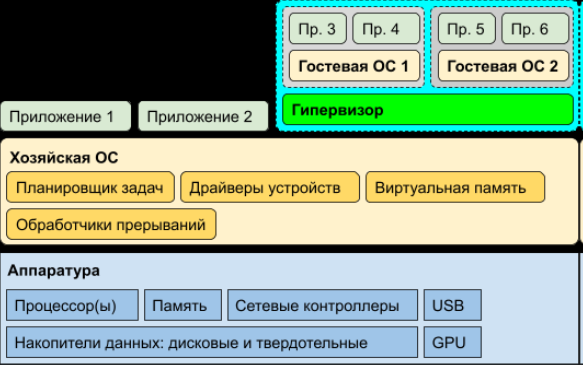
\includegraphics[width=1\textwidth]{1.png}}\\
    \small\textit{Архитектура DISCO, "Disco: Running Commodity Operating Systems on Scalable Multiprocessors",
    Edouard Bugnion, Scott Devine, and Mendel Rosenblum.}
    \label{framework} 
\end{figure}

Действительно, написание программного обеспечения (в том числе и операционных
систем), которое не только может эффективно использовать более одного
вычислительного устройства (процессора или процессорного ядра в многоядерных
системах), но и при этом еще и масштабируется (то есть продолжает так же
эффективно работать при большем или меньшем количестве вычислительных
устройств) является непростой задачей. Сложности возникают из-за необходимости
синхронизировать работу и программного обеспечения, выполняемого на разных
процессорах и некоторых внутренних состояний процессоров \footnote{\href{https://en.wikipedia.org/wiki/Synchronization_(computer_science)}{https://en.wikipedia.org/wiki/Synchronization\_(computer\_science)}}.\\

Если речь идет о прикладном программном обеспечении, то либо многопоточное
исполнение даже не требуется, либо, если есть возможность выполнять какие-то
операции параллельно, происходит работа с одними и теми же данными, иначе, мы
возвращаемся к первой ситуации когда более простое приложение выполняется в один
поток, а задача в целом решается запуском нескольких независимых однопоточных
приложений. То же, но еще в большей мере касается кода операционной системы: не
только происходит интенсивная работа с общими данными, которые описывают общие
состояния системы (время и дата, данные о пользователях, очередь задач и т.д.), но
еще добавляются одинаково доступные всем процессорам аппаратные ресурсы как-то:
внешняя память, порты ввода-вывода, сетевые контроллеры и т.п. Представьте себе,
что 2 процессора почти одновременно решили, что пора бы обновить системное
время, так как с момента последнего обновления уже прошла секунда. Однако, часы
реального времени (RTC) во всей системе только одни и, если оба процессора с
небольшой разницей во времени увеличат значение секунд на единицу, то фактически
время окажется установлено неправильно. Во избежание такой ситуации доступ к
разделяемым ресурсам сериализуется, то есть обеспечивается строго
последовательны доступ: пока один из процессоров работает с данным устройством,
все остальные находятся в состоянии ожидания, пока первый не закончит. И это
только самый простой и очевидный пример, на практике же наблюдается гораздо
больше и гораздо более сложных ситуаций для разрешения которых используются так
называемые синхронизационные примитивы. В свою очередь, синхронизационные
примитивы используют общие для всех процессоров данные и часто подразумевают
приостановку каких-то процессов до освобождения запрошенного ресурса.\\

Общие для нескольких процессоров данные порождают проблему когерентности этих
самых данных. То есть любой процессор в системе должен читать один и тот же байт
данных из памяти по адресу 0. И все было бы просто, если бы не сложность
современных процессоров, которые внутри имеют несколько кэшей \footnote{Кэш или кеш (англ. cache, от фр. cacher — «прятать») — промежуточный буфер с быстрым
доступом к нему, содержащий информацию, которая может быть запрошена с наибольшей
вероятностью. Доступ к данным в кэше осуществляется быстрее, чем выборка исходных
данных из более медленной памяти или удалённого источника, однако её объём существенно
ограничен по сравнению с хранилищем исходных данных. \\ \href{https://ru.wikipedia.org/wiki/Кэш}{https://ru.wikipedia.org/wiki/Кэш}} 
(а многие еще и иерархические) таких как кэши инструкций и данных, кэши блоков трансляции
виртуальных адресов в физические и т.д. И для поддержания когерентности данных
операционная система в некоторых случаях вынуждена сбрасывать эти кэши.
Сложности со сбросом кэша как минимум в том, что необходимо это не забывать
делать вовремя и в том, что чем чаще это делается, тем больше теряется
производительности системы - данные, ранее доступные в кэшах, приходится снова
вычитывать из медленной внешней памяти или даже заново вычислять.\\

И в очередной раз стоит вспомнить о важном аспекте - надежности системы. Имея в
виду сложности описанные выше, можно смело предположить, что ПО, реализующее
все необходимое для работы на многопроцессорной системе, является весьма
сложным и объемным. А это в свою очередь, означает, что вероятность присутствия в
таком ПО ошибок весьма велико. И как это ни печально, но крах операционной
системы неизбежно приводит к преждевременному завершения всех полезных задач,
которые были запущены поверх ОС.\\

Запуск нескольких экземпляров более простой ОС поверх гипервизора Disco был
призван помочь с решением обозначенных ранее проблем. Однако, стоит заметить,
что реально полезная работа, как правило, выполняется приложениями, запущенными
поверх ОС. А значит, при ограниченных аппаратных ресурсах, чем меньше ресурсов
уходит на работу ОС и гипервизора, тем больше остается полезным (будем надеяться,
что так) приложениям. И благодаря нескольким интересным техническим решениям
команде исследователей удалось добиться производительности приложений внутри
виртуальных машин лишь немного меньшей, чем при запуске на непосредственно на
аппаратуре.\\

Далее мы коротко рассмотрим наиболее интересные решения, которые реализовали в
гипервизоре Disco.\\

Исполнение команд гостевой системы непосредственно реальным процессором. Это
позволяет достичь максимальной производительности, неотличимой от запуска ПО без
гипервизора. Правда, есть один важный нюанс при непосредственном исполнении
команд гостя - не все команды гостя можно безопасно выполнять в присутствии
гипервизора. Например, только гипервизор должен иметь полный контроль над
состоянием процессора, в то время как гостевая система должна только "думать", что
она изменяет состояние процессора, но фактически важными (определенно, не всеми)
состояниями процессора должен управлять гипервизор (возможно, по "просьбе"
гостевой системы). Решение состоит в обнаружении и корректной симуляции 
таких критических операций. К счастью, такие операции случаются не слишком часто \footnote{Точнее, так любят писать в рекламных статьях разработчики гипервизоров. При этом обычно
приводятся результаты замеров, выполненных при запуске некоторых характерных тестов
как-то: SPEC INT2000, компиляция больших программных проектов, например, ядра ОС Linux и
т.п. Поскольку значительная часть вышеназванных задач состоит в вычислениях с
минимальным взаимодействием с аппаратурой, очевидно, абсолютное большинство команд
гостевой системы выполняются напрямую процессором и влияние гипервизора едва ли
заметно. Однако, стоит обратиться к задаче, которая более интенсивно взаимодействует с
аппаратурой (самого процессора или внешними устройствами), то можно запросто получить
ситуацию, когда гипервизор будет потреблять количество ресурсов соизмеримое с гостевой
системой. См. например, \href{https://www.cl.cam.ac.uk/research/srg/netos/papers/2003-xensosp.pdf}{https://www.cl.cam.ac.uk/research/srg/netos/papers/2003-xensosp.pdf}} 
и, потому, незначительно влияют на общую производительность системы.\\

Виртуальная физическая память \footnote{Для лучшего понимания, рекомендуется ознакомиться с концепцией виртуальной памяти
(\href{https://en.wikipedia.org/wiki/Virtual_memory}{https://en.wikipedia.org/wiki/Virtual\_memory}) и ее реализацией в современных процессорах при
помощи MMU (Memory Management Unit - \href{https://en.wikipedia.org/wiki/Memory_management_unit}{https://en.wikipedia.org/wiki/Memory\_management\_unit}).}. Гостевая система, использующая концепцию
виртуальной памяти (а таковы все современные ОС общего назначения),
предполагает, что она имеет доступ ко всей физической памяти, имеющейся в системе
и может программировать MMU для трансляции виртуальных адресов в физические по
своему усмотрению. Более того, гостевые системы даже не подозревают, что вместе с
ними на той же аппаратуре могут работать еще и другие гости, которые точно так же
хотят программировать MMU. Таким образом неизбежны коллизии между гостевыми
системами из-за перепрограммирования MMU (первый гость программирует MMU на
трансляцию виртуального адреса 0 в физический адрес 0x1000, а второй гость
перепрограммирует MMU так, чтобы виртуальный адрес 0 транслировался в
физический адрес 0x8000). Решение состоит в том, что гипервизор обнаруживает
попытку запрограммировать MMU гостем и программирует MMU самостоятельно, но с
учетом уже имеющихся трансляций для других гостей.\\

Диски с "копированием-при-записи" \footnote{\href{https://en.wikipedia.org/wiki/Copy-on-write}{https://en.wikipedia.org/wiki/Copy-on-write}}. Эта техника позволяет избежать повторного
чтения данных с диска, если ранее эти данные были уже прочитаны и все еще
находятся в памяти. Таким образом, значительно повышается эффективность
использования дисковой подсистемы. Идея в том, что при наличии нескольких гостей,
использующих одно и то же программного обеспечение, можно считывать данные и,
собственно, код ПО с диска только в первый раз, а затем для других гостей при
помощи MMU делать эти данные доступными другим гостям. Тут важно помнить, что
каким бы быстрым ни был внешний накопитель, данные нужно сначала загрузить в
память, а потому отсутствие чтения со внешнего накопителя как минимум вдвое
уменьшает время доступа процессора к данным.\\

Виртуальный сетевой интерфейс для взаимодействия гостевых систем друг с другом.
Поскольку, данные, которыми обмениваются гостевые системы, не покидают пределов
одной физической машины, то вместо пересылки данных можно использовать буфера
в памяти, доступные обоим гостям, тем самым снова исключаются дополнительные
копирования данных.\\

Как и в случае с изобретением виртуальной машины компанией IBM, мы
обнаруживаем, что в Disco нашли свое воплощение идеи, которые и по сей день
используются в самых современных системах виртуализации.\\

Тем не менее, Disco навсегда остался интересным исследовательским проектом.
Однако, его авторы нашли применение полученным знаниям: 10 февраля 1998 была
основана компания VMware, а в мае 1999 года был выпущен первый продукт компании
VMware Workstation. Несколько удивительным может показаться то, что первый
продукт компании оказался нацелен на рынок виртуализации рабочих станций, а вовсе
не серверов, хотя, казалось бы, предыдущий опыт был связан именно с серверами и
повышением эффективности использования аппаратуры. Хотя, если вникнуть в
детали, то гораздо более любопытным оказывается совсем другой факт: VMware
Workstation обеспечивал запуск виртуальной машины на процессорах Intel (которые,
будучи разработанными несколько десятилетий спустя IBM 360, не удовлетворяли
требованиям эффективной виртуализации - мы рассмотрим это позже).\\

В 2001 году VMware представила сразу 2 продукта для серверов: VMwa- re GSX Server
and VMware ESX Server\footnote{Согласно Майку ДеПетрилло (Mike DiPetrillo, \href{https://vimeo.com/10733576}{https://vimeo.com/10733576}) - одному из
старожилов VMware, GSX - это сокращение от Ground Storm X, а ESX - сокращение от Elastic
Sky X. При этом буква "X" не значила ровным счетом ничего, а лишь добавляла "крутости"
звуанию. Что же касается "Ground Storm" и "Elastic Sky" - то доподлинно неизвестно, кто и
почему выбрал такие словосочетания.}. Оба продукта во многом базировались 15 на технических
решениях, обкатанных на VMware Workstation.\\

Позже в 2003-м году добавились сопутствующие продукты для управления
виртуальными машинами - VMware Virtual Center и vMotion, а в 2007-м году был
выпущен новый продукт VMware ESXi (ESX integrated\footnote{Несколько странным выглядит термин "интегрированный" (integrated), при том, что ESXi
изначально был сильно облегченным ESX (дистрибутив размером всего 32 МБ вместо более
чем гигабайта полного ESX, имевшего Red Hat Enterprise Linux в качестве "Service Console").
Однако, речь идет об интеграции в сам гипервизор сервисной консоли в виде популярного во
встраиваемых системах набора утилит Busybox (\href{https://busybox.net/}{https://busybox.net/}).}).\\

В настоящее время компания VMware занимает позицию лидера на рынке серверной
виртуализации со значительным отрывом от ближайших конкурентов. Это оказалось
возможным благодаря значительному опыту и инновациям, которые позволяют
компании выпускать чрезвычайно эффективные решения для виртуализации серверов
и рабочих станций, а также предлагают инструменты управления виртуализованной
инфраструктурой.

\subsection*{Virtual PC: Connectix, Microsoft, Windows}
\addcontentsline{toc}{subsection}{Virtual PC: Connectix, Microsoft, Windows}

Как мы увидели, корпорации такие как IBM и академические учреждения такие как
Стэнфордский университет продававшие или использовавшие огромные
вычислительные машины, мэйнфреймы, были, очевидно, озабочены более
эффективным их использованием, а потому активно развивали серверную виртуализацию. Но к концу 20-го столетия уже вовсю расцвели персональные
компьютеры и виртуализация нашла себе еще одно применение - возможность
запускать на одном и том же компьютере одновременно несколько разных
операционных систем. В противном случае несчастный (или наоборот счастливый)
владелец компьютера Apple, разумеется, с MacOS не мог запустить программное
обеспечение, существовавшее только в версии для Windows, OS/2 или же Red Hat
Linux.\\

В середине 80-х годов Род МакГрегор (Rod MacGregor, впоследствии основавший
компанию Insignia Solutions) разработал программный эмулятор процессоров Intel с
архитектурой x86. Таким образом, сделав возможным выполнение программ
скомпилированных для процессоров Intel на самой разнообразной аппаратуре:
изначально речь шла о рабочих станций с UNIX, а затем в 1987 году появилась версия
и для Apple Macintosh II\footnote{В журнале"MacWorld" за октябрь 1987 года говорилось "Люди, желавшие пользоваться MS
DOS, были вынуждены покупать IBM PC или совместимые с ними компьютеры - теперь же они
могут запускать MS DOS прямо на своих Маках". В переводе на деньги это значило, что вместо
покупки IBM PC совместимого компьютера за \$1500 можно было купить эмулятор SoftPC всего
за \$595 (естественно, это все в случае, если у кого-то уже был во владении Apple Mac II).\href{https://archive.org/stream/MacWorld_8710_October_1987/page/n11/mode/2up}{https://archive.org/stream/MacWorld\_8710\_October\_1987/page/n11/mode/2up}}.\\

Теперь вдохновленные успехом SoftPC и другие компании начали задумываться о
подобных продуктах. Одной из таких стала компания Connectix \footnote{История компании Connectix весьма интересна и печальна. Интересна потому, что она была
настоящим инноватором: разработала и производила первую в мире веб-камеру, названную
QuickCam; разработала Virtual PC, ставший сначала виртуальной машиной по умолчанию в
Microsoft Windows, и послужившая отправной точкой в разработке гипервизора нового
поколения Microsoft Hyper-V; разработала эмулятор Sony PlayStation и т.д. А печальна потому,
что компания Apple вдохновляясь продуктами Connectix, интегрировала аналогичные решения
в свою операционную систему, делая утилиты Connectix никому более не нужными;
продуктовая линейка вэб-камер QuickCam была выкуплена компанией Logitech в 1998 году;
программный эмулятор Sony Playstation "Connectix Virtual Game Station" после неудачного
судебного решения в пользу Connectix был выкуплен компанией Sony и тут же предан
забвению; а в 2003 году вместе с покупкой Virtual PC, прекратила свое существование и сама
компания Connectix.} с продуктом под названием Virtual PC. Первоначально, 
представленное в июне 1997 года, Virtual PС было приложением для System 7.5 \footnote{Теперь бы мы назвали ее Apple MacOS 7.5.} 
и позволяло установить и запустить ОС WIndows
на компьютерах Apple. Позже в 2001 году версия 4,0 имела уже поддержку
компьютеров с ОС Windows, позволяя на них запускать OS/2 или Red Hat Linux.\\

Как известно, компания Microsoft никогда не изобретала совершенно новых продуктов,
предпочитая ворваться на уже существующий рынок и занять на нем доминирующее
положение, взяв за основу какой-то уже существующий продукт. Так произошло и с
виртуализацией - вместо разработки с нуля своего решения, Microsoft в 2003 году
купила уже весьма популярный Virtual PC вместе с командой, которая этот продукт
разрабатывала и поддерживала (тем самым закончив историю компании Connectix).
Так появился Microsoft Virtual PC. А вместе с выпуском Windows 7, был анонсирован
еще раз переименованный продукт Windows Virtual PC. Тем не менее, начиная с Windows 8 компания Microsoft заменила Virtual PC совершенно новым решением для
виртуализации - Microsoft Hyper-V, но о нем немного позже.

\subsection*{VirtualBox: Innotec, Sun, Oracle}
\addcontentsline{toc}{subsection}{VirtualBox: Innotec, Sun, Oracle}

В 2002 году компания Innotec GmbH по соглашению с Connectix Corporation создала
версию Virtual PC для OS/2 (интересно то, что IBM не занималась обновлением OS/2 с
1996 года, когда вышла OS/2 Warp 4). А в 2007 году компания Innotec GmbH выпускает
свой собственный продукт Innotec VirtualBox - вот так сюрприз!
В 2008 году компания Innotec GmbH была приобретена компанией Sun Microsystems, а
та, в свою очередь, была приобретена компанией Oracle Corporation в январе 2010
года. Так появился продукт под названием "Oracle VM VirtualBox".

\subsection*{Xen}
\addcontentsline{toc}{subsection}{Xen}

Еще один исследовательский проект (в данном случае ведомый Яном Праттом из
компьютерной лаборатории Кембриджского университета), превратившийся в
настоящее энтерпрайз решение. Xen (по сути минималистичный
кросс-платформенный гипервизор первого типа) был разработан в момент, когда уже
накопилось достаточно опыта в виртуализации для процессоров Intel x86 \footnote{Первая стабильная версия Xen была анонсирована в октябре 2003 года -
\href{https://lwn.net/Articles/52033/}{https://lwn.net/Articles/52033/}}, а потому,
удалось достичь высочайшей для того времени эффективности работы гипервизора и
изоляции ресурсов. Во всяком случае, заявлялось, что накладные расходы на работу
гипервизора Xen составляют лишь единицы процентов, что является значительно
лучшим результатом по сравнению, во всяком случае, с VMware Workstation and User
Mode Linux.\\


Одна из важных особенностей гипервизора Xen — это поддержка режима
паравиртуализации, то есть запуска специальным образом модифицированных ОС
или их частей. И как мы позже увидим, паравиртуализация позволяет добиться
максимальной эффективности системы виртуализации.
На сегодняшний гипервизор Xen существует и развивается как проект с открытым
исходным кодом под эгидой организации Linux Foundation и является основой сразу
нескольких коммерческих продуктов, таких как Citrix XenServer, Oracle VM Server for
x86 и Huawei FusionSphere.

\subsection*{KVM}
\addcontentsline{toc}{subsection}{KVM}

Поскольку гипервизор является самым низкоуровневым программным обеспечением,
которое работает непосредственно с аппаратурой, то при его разработке приходится
обязательно реализовывать подпрограммы управления используемой аппаратурой:
таймеров, контроллеров прерываний, MMU, устройств ввода-вывода и т.д.\\


Во-первых, обслуживание названных аппаратных блоков зачастую оказывается весьма
непростым: сложной может оказаться и логика работы устройства и количество
режимов работы более одного и т.д. А во-вторых, при адаптации гипервизора к каждой 
новой аппаратной системе приходится добавлять поддержку все новых и новых
компонентов. Так почему бы не воспользоваться тем, что уже сделано? Например,
можно взять ядро операционной системы с открытым исходным кодом такое как Linux,
в котором есть поддержка огромного количества аппаратуры (только разных
процессорных архитектур поддерживается более десятка) и просто добавить
функциональность, которой не хватает для реализации режима гипервизора.\\

Собственно, так и поступил Ави Кивити (Avi Kivity) из стартапа под названием
Qumranet, который в 2008 году был приобретен компанией Red Hat. Таким образом,
начиная с версии 2.6.20 ядро ОС Linux может выступать в роли полноценного
гипервизора. Более того, в отличие от других гипервизоров первого типа, KVM может
быть запущен на любой аппаратуре, для которой существует порт ядра Linux \footnote{Подразумевается, что архитектура процессора данной системы имеет поддержку KVM. На
сегодняшний день это как минимум: x86, IBM S/390, PowerPC и ARM.}, что
делает его особенно популярным среди исследователей, некоммерческих и
образовательных учреждений и стартапов.

\subsection*{Microsoft Hyper-V}
\addcontentsline{toc}{subsection}{Microsoft Hyper-V}

Несмотря на то, что у компании Microsoft было готовое решение для виртуализации
(упомянутый выше Virtual PC), было принято решение создать новый более
современный гипервизор с нуля. Дело в том, что Virtual PC все-таки работал поверх
основной операционной системы и потому был менее эффективен по сравнению с
конкурирующими решениями, где использовался гипервизор первого типа
(запущенный непосредственно на аппаратуре без дополнительных прослоек
программного обеспечения). Так в октябре 2008 года миру был явлен гипервизор
Microsoft Hyper-V, который с тех пор прошел уже значительный путь от не слишком
стабильного нововведения до одного из лидеров в серверной виртуализации: не
только множество компаний по всему миру используют Hyper-V как базовый
гипервизор, но и сама Microsoft использует Hyper-V в сердце своей облачной
инфраструктуры Azure.\\

\noindent {\Large \slshape{Немного терминологии}}\\

\noindent Для того чтобы говорить на одном языке с читателем, перво-наперво предлагаю
ознакомиться с наиболее важными и часто встречающимися в данном курсе
терминами.\\

\noindent {\large \slshape{Гостевая система}}\\

\noindent \underbar{Гостевая система} (от англ.guest - гость) - виртуальная, симулируемая система,
запущенная под управлением гипервизора или симулятора, а также работающее
контейнеризованное окружение.\\

\noindent {\large \slshape{Гипервизор}}\\

\noindent \underbar{Гипервизор или монитор виртуальных машин} - программное обеспечение, запущенное
на хозяйской системе, позволяющее создавать и управлять виртуальными машинами.

\section*{Задачи решаемые при помощи виртуализации}
\addcontentsline{toc}{section}{Задачи решаемые при помощи виртуализации}

Как мы могли видеть из исторического обзора систем виртуализации, все началось с
несколько необычной реализации многопользовательской операционной системы на
мэйнфреймах IBM, а на сегодняшний день сосуществуют множество весьма разных
систем виртуализации на любой вкус. Более того, виртуальные машины находят свое
применение в самых разных областях науки и техники, порой, даже несколько
необычных таких как автомобили, телекоммуникационное оборудование т.д. Если мы
разберемся, в решении каких задач могут быть использованы виртуальные машины, то
станет понятна мотивация их использования в конкретных областях и случаях.

\subsection*{Эффективное использование аппаратуры (partitioning)}
\addcontentsline{toc}{subsection}{Эффективное использование аппаратуры (partitioning)}

Именно желание повысить эффективность использования дорогостоящей аппаратуры
послужило толчком к созданию первой виртуальной машины инженерами IBM. Идея до
безобразия проста: если аппаратура имеет достаточно ресурсов, чтобы одновременно
исполнять несколько задач, то почему бы эти несколько задач и не выполнять? В
случае использования только аппаратуры можно легко себе представить едва ли
решаемую проблему: как быть, если из двух программ, которые нужно одновременно
выполнять, одна требует наличия Windows, а вторая Ubuntu? Если же на аппаратуре
запущен гипервизор, а поверх него 2 гостевые системы с Windows и Ubuntu, то проблема оказывается решенной. Однако, виртуализация может оказаться полезной
даже при запуске виртуальных машин с одинаковой системой внутри. Более того, при
использовании идентичных систем в разных виртуальных машинах, можно обеспечить
еще и более высокую производительность системы в целом за счет
переиспользования общих страниц памяти с кодом и данными.

\begin{figure}[h]
    \centering
    \scalebox{0.75}{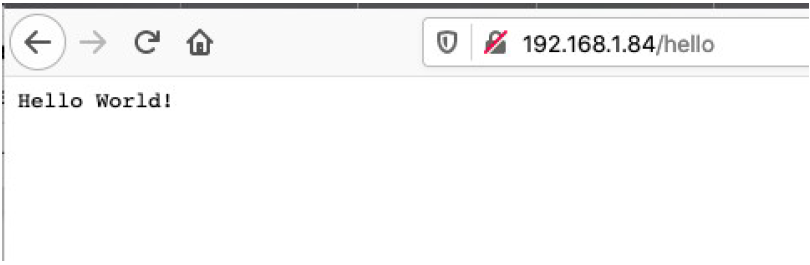
\includegraphics[width=1\textwidth]{2.png}}
    \label{framework} 
\end{figure}

\subsection*{Абстрагирование от аппаратуры}
\addcontentsline{toc}{subsection}{Абстрагирование от аппаратуры}

Первоначально определение термина "виртуальная машина" было дано Геральдом
Попеком и Робертом Голдбергом в их статье 1974 года "Формальные требования к
виртуализируемым архитектурам третьего поколения\footnote{ЭВМ 3-го поколения - это машины, разработанные в 60-70-х годах 20-го века, построенные на
базе интегральных схем в противовес ранее использовавшимся транзисторам и электронным
лампам.}"\footnote{\href{"Formal Requirements for Virtualizable Third Generation Architectures"}{"Formal Requirements for Virtualizable Third Generation Architectures"}} в следующем виде:
"эффективная и изолированная копия реального компьютера". С тех пор определение
несколько поменялось в том смысле, что вовсе не обязательно речь идет о копии
некоего реального компьютера. И, действительно, современные виртуальные машины
могут создавать такое окружение для запуска гостевой системы, что гостевая система
будет работать так, как если бы она была запущена совершенно на другой аппаратуре
- значительно отличающейся от реально используемой машины. Другими словами,
гипервизор позволяет абстрагироваться от реальной аппаратуры.

\subsection*{Создание предсказуемого окружения}
\addcontentsline{toc}{subsection}{Создание предсказуемого окружения}

Казалось бы, зачем идти на такое усложнение: имея в реальной системе аппаратный
блок А, для гостевой системы делать вид, что вместо блока А присутствует блок Б.
Например, в моей системе установлен современный высокоскоростной сетевой
контроллер "Intel I219-V Ethernet", а Oracle VirtualBox и VMware Workstation по
умолчанию для гостей эмулируют древний "AMD PCNet".
Ответ состоит в том, что независимо от реальной конфигурации компьютера,
виртуальная машина будет работать в одинаковом окружении. Это дает как минимум
две интересных возможности: во-первых, один и тот же образ виртуальной машины
можно одинаково использовать и на своем компьютере и на компьютере соседа, то
есть обеспечивается переносимость виртуальной машины, а во-вторых, заранее зная
конфигурацию виртуального окружения, можно подготовить программное обеспечение
гостевой системы так, чтобы оно соответствовало окружению\footnote{Например, можно заранее интегрировать все необходимые драйвера в образ гостевой
операционной системы и не заниматься их установкой во время первого старта системы.} или наоборот, зная,
какую аппаратуру поддерживает гостевая ОС, можно сконфигурировать виртуальное
окружение для эмуляции именно поддерживаемой аппаратуры.
Или можно описать стандарт окружения и гостевой ОС и наслаждаться
беспроблемным использованием гостевых систем в стандартных виртуальных
машинах.

\subsection*{Повышение безопасности}
\addcontentsline{toc}{subsection}{Повышение безопасности}

Несмотря на то, что современные операционные системы общего назначения
используют концепцию виртуальной памяти и каждый запущенный в системе процесс
выполняется с своем уникальном адресном пространстве, все еще существует
множество способов для злонамеренной (или же просто неграмотно написанной)
программы повлиять не только на выполнение других процессов, но даже привести к
краху самой операционной системы. Однако, если разделить все необходимое
программное обеспечение на несколько частей и запускать их на разных виртуальных
машинах, то в результате гораздо более надежной изоляции, той самой плохо
написанной программе будет гораздо сложнее повлиять на ход выполнения
программного обеспечения в соседней виртуальной машине\footnote{Важно помнить о том, что не существует способа изоляции процессов друга от друга более
надежного, чем запуск этих процессов на разных машинах, которые не имеют совершенно
никаких связей: ни по сети обмена данными, ни посредством оператора, ни через сеть 220В. А
посему не стоит наивно верить в рассказы производителей аппаратуры и ПО о чудесных
свойствах их виртуальных машин.}.
Более того, гипервизор может не только управлять ресурсами хозяйской системы, но и
следить за тем, какой код выполняется в гостевых системах и при обнаружении
опасных команд или их последовательностей, может исполнять их безопасным
образом.

\subsection*{Повышение надежности}
\addcontentsline{toc}{subsection}{Повышение надежности}

Все сказанное выше о безопасности в полной мере применимо и к вопросам
обеспечения повышенной надежности. Во-первых, изолируя гостевые системы, мы
автоматически значительно снижаем возможности для их влияния друг на друга.
Во-вторых, жестко регламентируя количество ресурсов, доступных конкретной
гостевой системе, можно гарантировать наличие достаточных ресурсов для этогй и/или
других гостевых систем. То есть, если каждой гостевой системе дано в использование
одно процессорное ядро реального компьютера, то как бы жадный до вычислительных
ресурсов процесс одной гостевой системы того не хотел, он не сможет использовать
ресурсы других вычислительных ядер. Более того, как мы увидим позже,
виртуализация сделала возможным незаметный перенос гостевой системы с одного
физического сервера на другой, в том числе при обнаружении проблем с аппаратурой
первоначально используемого сервера.

\subsection*{Облачные вычисления}
\addcontentsline{toc}{subsection}{Облачные вычисления}

И, наконец, мы не можем не упомянуть облачные вычисления или облачные сервисы.
Благодаря особенностям, перечисленным ранее, виртуализация сделала возможным
предоставление удаленных вычислительных ресурсов, хранилищ данных,
программных продуктов или даже целых IT-инфраструктур. Действительно, на некоем
реальном сервере можно запускать любое сколь угодно сложное программное
обеспечение в изолированном окружении, которое контролируется гипервизором. И таких окружений может быть множество; имеющиеся аппаратные ресурсы можно
динамически перераспределять в зависимости от потребности клиентов; клиенты и
владельцы сервера могут пребывать в относительном спокойствии касательно
сохранности своих данных.

\section*{Требования, применяемые к виртуальным машинам}
\addcontentsline{toc}{section}{Требования, применяемые к виртуальным машинам}

Перед тем как мы начнем рассматривать особенности конкретных гипервизоров и
виртуальных машин, имеет смысл сформулировать требования, которым хорошая
виртуальная машина должна удовлетворять. Иначе, невелика цена такой виртуальной
машине.\\

Как мы помним, изобретение виртуализации случилось еще 60-х годах прошлого века,
а в последующие годы проводилось достаточно научных изысканий на тему
виртуализации. Одной из важнейших работ оказалась статья Геральда Попека и
Роберта Голдберга "Формальные требования к виртуализируемым архитектура
третьего поколения", опубликованная в 1974 году. В ней в частности говорилось о
желаемых свойствах виртуальных машин и формулировались требования к
канонически правильно виртуализуемой процессорной архитектуре.

\subsection*{Безопасность, эквивалентность, эффективность}
\addcontentsline{toc}{subsection}{Безопасность, эквивалентность, эффективность}

По определению, виртуальная машина должна вести себя так же как и реальная
машина, будь-то: некий конкретный компьютер, если речь идет о эмуляции строго
заданной системы, или некоторая абстрактная аппаратура. Таким образом можно
сформулировать следующие требования к современному гипервизору:
\begin{enumerate}
    \item Гипервизор должен обладать возможностью полного контроля над
    виртуализованными ресурсами, таким образом обеспечивая безопасность для
    гостевых и хозяйской систем.
    \item Программное обеспечение, запущенное в виртуализованном окружении должно
    вести себя в точности так же, как если бы оно было запущено на реальной
    аппаратуре.
    \item Гипервизор, не выполняя никакой полезной работы, должен использовать как
    можно меньше ресурсов хозяйской системы, оставляя максимум ресурсов
    гостевым системам, то есть гипервизор должен быть как можно более
    эффективным.
\end{enumerate}

\subsection*{Критерий виртуализации Попека-Гольдберга}
\addcontentsline{toc}{subsection}{Критерий виртуализации Попека-Гольдберга}

В своей работе Попек и Голдберг выдвинули в числе прочих следующую теорему:
полноценный гипервизор для данной процессорной архитектуры может быть
реализован только в том случае, если набор служебных команд является
подмножеством привилегированных команд.\\

Привилегированными называются такие команды процессора, которые могут
нормально исполняться только в привилегированном режиме работы процессора, а
будучи вызванными в непривилегированном режиме работы, приводят к
возникновению исключительной ситуации, для обработки которой процессор
автоматически переключается в привилегированный режим. Служебными же (или
"чувствительными" в терминологии Попека и Голдберга) командами называются такие
команды процессора, которые могут повлиять на работу гипервизора. Например, к
таким командам можно отнести команды управления MMU или команды, управляющие
прерываниями.\\

Таким образом, если все служебные команды являются еще и привилегированными,
то попытка их исполнения в гостевой системе приведет к возникновению
исключительной ситуации, управление будет передано гипервизору, который сможет
обработать данную команду по своему усмотрению, а затем управление вернется
гостевой системе, которая продолжит свое исполнение как ни в чем не бывало.
Однако, если данное условие не выполняется, то гостевая система сможет повлиять
на работу гипервизора, тем самым лишив его контроля за происходящим, и перевести
всю систему в совершенно нежелательное состояние.\\

Просто удивительно, что лишь некоторые процессоры Intel и только начиная с 2005
года будут соответствовать этому требованию.

\section*{Вопросы лицензирования}
\addcontentsline{toc}{section}{Вопросы лицензирования}

В очередной раз возвращаясь к определению виртуальной машины, мы вспоминаем,
что виртуальная машина должна вести себя как копия некоторой реальной машины. И
уже это само определение таит в себе некоторые сложности, когда речь заходит о
запуске лицензируемого программного обеспечения. Потому стоить уделить немного
внимания этим вопросам.

\subsection*{Проприетарное ПО}
\addcontentsline{toc}{subsection}{Проприетарное ПО}

При том, что виртуальная машина может действительно быть копией реального
компьютера (точнее быть цифровым образом программного обеспечения и данных
того компьютера), многое проприетарное программное обеспечение требует получения
отдельной лицензии на каждую свою копию. То есть, в общем случае запуск
проприетарного ПО внутри виртуальной машины требует получения лицензии для
каждого экземпляра данной программы, даже в случае запуска нескольких клонов
(бинарных копий) одной и той же виртуальной машины. И все это при том, что
виртуальная машина не является физически еще одним компьютером, но тем не
менее даже программа, запущенная внутри программы (гипервизора) может требовать
полноценной лицензии.\\

Однако, может быть еще хуже — лицензионное соглашение на ПО может либо
полностью запрещать использование данного ПО в виртуальных машинах, либо не
давать ясного понимания ограничений и требований. В таком случае стоит либо
обратиться с вопросами к разработчику такого ПО, либо вовсе отказаться от
использования данного ПО в виртуальных машинах.

\subsection*{Привязка лицензии к аппаратуре}
\addcontentsline{toc}{subsection}{Привязка лицензии к аппаратуре}

Еще более сложной может оказаться ситуация, когда лицензия привязывается к
каким-то особенностям аппаратуры, как-то: серийный номер какого-то компонента,
MAC-адрес сетевой карты, внешний криптографический USB-ключ и т.д. Во-первых, в
некоторых виртуальных машинах необходимый аппаратный компонент может
отсутствовать. Думаю, легко представить сложности с использованием USB-ключа с
программой, запущенной в облачном сервисе — у пользователя с большой
вероятностью не будет физического доступа к серверу, на котором исполняется его
программа. Во-вторых, свойства необходимого аппаратного компонента, видимые из
виртуальной машины, могут в точности совпадать с таковыми реальной аппаратуры.
При том, что это в теории может сделать возможным использование той же лицензии,
что была получена для реальной аппаратуры, и в виртуальных машинах. На практике
это может нарушать лицензионное соглашение, которое может требовать получение
отдельной лицензии для каждого экземпляра программы или машины (физической или
виртуальной).

\subsection*{Повторное использование лицензии}
\addcontentsline{toc}{subsection}{Повторное использование лицензии}

Отдельные вопросы возникают в случае, когда виртуальные машины создаются по
требованию:
\begin{itemize}
    \item Как вести учет лицензиям в динамически создаваемых виртуальных машинах?
    \item Можно ли заново использовать лицензию с только что уничтоженной
    виртуальной машины на заново создаваемой?
    \item К чему привязывать лицензию, если параметры виртуальных машин либо
    назначаются случайным образом, либо одинаковы на всех машинах?
\end{itemize}

Ввиду обозначенной выше неразберихи и неоднозначности, имеет смысл соблюдать
особенную осторожность при использовании проприетарного ПО на виртуальных
машинах и стараться прояснять любые неочевидные ситуации с производителем ПО
или его локальным представителем.

\section*{Использованные источники информации}
\addcontentsline{toc}{section}{Использованные источники информации}

\begin{enumerate}
\item "Современные операционные системы", 4-е издание, Э. Таненбаум, Х. Бос
\item "History of Virtualization", Sean Conroy \href{https://www.idkrtm.com/history-of-virtualization/}{\textit{\underbar{https://www.idkrtm.com/history-} \underbar{of-virtualization/}}}
\item "Evolution of a Virtual Machine Subsystem", 1979 article by Edson C. Hend- ricks and
T.C. Hartmann in IBM Systems Journal, Vol. 18. No. 1, 1979, pp. 111-142, provided
by George McQuilken, former editor of IBM Systems Journal. \href{https://pdfs.semanticscholar.org/72a5/c6dd54e3dbb64f8a48ed9f968bb740639c0d.pdf}{\textit{\underbar{https://pdfs.semanticscholar.org/72a5/c6dd54e3dbb64f8a48ed9f9}\\\underbar{68bb740639c0d.pdf}}}
\item Edouard Bugnion; Scott Devine; Kinshuk Govil; Mendel Rosenblum (Nove- mber
1997). "Disco: Running Commodity Operating Systems on Scalable Multiprocessors" \ \
 \href{https://web.archive.org/web/20120813061150/http://www.stanford.edu/class/cs240/re
adings/disco.pdf}{\textit{\underbar{https://web.archive.org/web/20120813061150/http://w}\\\underbar{ww.stanford.edu/class/cs240/re
adings/disco.pdf}}}
\item "Cloud Computing, Theory and Practice", Dan C. Marinescu \href{https://eclass.uoa.gr/modules/document/file.php/D416/CloudComputingTheoryAndPr
actice.pdf}{\textit{\underbar{https://eclass.u}\\\underbar{oa.gr/modules/document/file.php/D416/CloudComputingTheoryAndPract}\\\underbar{ice.pdf}}}
\end{enumerate}


\end{document}